\documentclass[11pt]{article}
\usepackage[a4paper,margin=2.5cm]{geometry}
\usepackage{graphicx}
\usepackage{booktabs}
\usepackage{amsmath,amssymb}
\usepackage[hidelinks]{hyperref}
\graphicspath{{../data/}}
\newcommand{\Tobs}{T_{\rm obs}}
\newcommand{\Cobs}{C_{\rm obs}}
\newcommand{\psig}{p_{\rm sig}}
\newcommand{\pnull}{p_{\rm null}}
\newcommand{\ppers}{p_{\rm persist}}

\title{The published 741-day light-curve formula of the quasar SDSS~J0159+0105 fails on held-out ZTF data; post hoc, a weaker persistent 741-day signal is not excluded}
\author{Qianghao Wu}
\date{28 November 2026}

\begin{document}
\maketitle

\begin{abstract}
\noindent Zheng et al.\ (2016) reported two periodic signals, at about 741 and 1500 days, in the 8.1-year Catalina (CRTS) V-band light curve of the radio-quiet quasar SDSS J0159+0105 ($z = 0.217$), and proposed a supermassive black hole binary. They gave the 741-day signal as a formula: $V = 0.1 \sin(2\pi(t - 53413.09)/741) + 16.59$. Their data end in 2013. Before we downloaded any later data, we registered a test of this formula on public Zwicky Transient Facility (ZTF) g and r data from June 2018 to October 2025 (2448 points, 2.3 to 5.9 cycles after the last CRTS point). The fitted amplitude of the continued formula is $T = -0.59$, where the formula predicts $T = 1$. In 5000 simulations of the formula plus damped-random-walk red noise, none gives $T \le -0.59$ ($p < 2\times10^{-4}$; power 0.82). By the registered rule, the formula at its published amplitude, period and phase is refuted. A part of this failure is not new: the 252 CRTS points that we read from the paper's own figure give a 741-day amplitude of 0.050~mag, half of the published 0.1~mag. The new information from ZTF is the sign of $T$. Post hoc, we also tested a persistent sinusoid whose period, amplitude and phase are refitted to the CRTS points in each simulation. The period of this refit has a scatter of 15 to 72~d, so its phase at the ZTF epochs is uncertain by 0.1 to 0.8 cycle. Such a signal gives a ZTF result as low as the observed one in 0.6\% to 9.8\% of simulations over eight noise models. So a persistent signal near 741 days is not refuted. Red noise alone gives the observed result in 20\% of simulations, so the ZTF data give no evidence for the signal either. The 1500-day signal is not tested. This work has not yet been reviewed by experts. The computations and the text were produced by AI models (from Anthropic and OpenAI), working under the author's direction.
\end{abstract}

\section{Introduction}

Two supermassive black holes in a close orbit can change the accretion rate of the surrounding gas with the orbital period. A quasar whose brightness changes periodically is therefore a candidate binary. But all quasars vary at random. Their optical variability is red noise, and a damped random walk (DRW) describes it well \cite{kelly2009,macleod2010}. A few cycles of red noise can look periodic, so a period that rests on few cycles is weak evidence \cite{vaughan2016}. A real period continues after the data that found it. A chance pattern usually does not. A test on data taken after the discovery is therefore the most direct check of a candidate.

Zheng et al.\ (2016) searched the Catalina Real-time Transient Survey (CRTS) \cite{drake2009} V-band light curves of 347 bright low-redshift quasars in SDSS Stripe 82 for periodic signals \cite{zheng2016}. They used a Lomb--Scargle code with a DRW noise model (GLSdeDRW) and an autocorrelation analysis. In the quasar SDSS J015910.058+010514.53 (J0159, $z = 0.217$; not the changing-look quasar SDSS J015957.64+003310.5, which some papers also call SDSS J0159) they found, in their words, ``two significant (at $P>99\%$) periodic signals at $\sim$741 day and $\sim$1500 day from the 8.1-year Catalina V-band light curve''. Their Section~4.1 gives the shorter signal as an explicit curve: ``Only the sinusoidal signal, which can be fitted as $V$ = 0.1 $\times$ sin(2$\pi$(t - 53413.09)/741) + 16.59 [\dots], is also confirmed by the additional ACF analysis ($P>99\%$).'' Here $t$ is the Modified Julian Date (MJD). The 1497-day signal comes from the autocorrelation analysis alone, and the paper gives no curve for it. The authors identified the 2:1 ratio of the two periods with a ratio that simulations of circumbinary disks predict, and took 1497~d as the orbital period.

Two later papers by other authors discuss this candidate. Charisi et al.\ (2018) tested the relativistic Doppler-boost model on CRTS candidates \cite{charisi2018}. Their footnote~1 states that J0159 was in the sample of Graham et al.\ (2015) \cite{graham2015}, and that its ``shortest periodic component of $\sim$740 d was identified with both the wavelet and the autocorrelation function analysis in G15, but did not have enough power to be classified as periodic''. Their test uses the CRTS data only. The review of D'Orazio and Charisi (2023) lists J0159 among the individually identified optical candidates: ``It has two periods (741 and 1500 days) and was interpreted as having the predicted by simulations 2:1 period ratio'' \cite{dorazio2023}. A related population test exists: El-Badry, Hogg and Rix (2026) continued the periodic models of 181 Gaia DR3 candidates into ZTF and CRTS data, and found that in all 116 cases with ZTF data the model fails to predict the later variability \cite{elbadry2026}. J0159 is not in their list: the nearest of their 116 Gaia sources is 6.5 degrees away.

We found no test of J0159 on data taken after 2013. The search covered the works that cite Zheng et al.\ in Semantic Scholar (38) and OpenAlex (82), two public archives of AI-produced results, and web searches (Section~\ref{sec:prior}).

This paper gives a forward test of the published 741-day formula on public ZTF data \cite{bellm2019,masci2019}. Section~\ref{sec:method} gives the registered test. Section~\ref{sec:result} gives its result. Section~\ref{sec:posthoc} gives tests that we added after we saw the result: a control on the CRTS data of the paper, and a test of a persistent sinusoid with the period-fit error included.

\section{Data}

\paragraph{ZTF.} We downloaded the ZTF light curves from the NASA/IPAC Infrared Science Archive (IRSA) light-curve service, in a 2.2-arcsec circle around RA 29.791908, Dec $+1.087369$. We kept all zg and zr points with \texttt{catflags} $= 0$. The sample has 2448 points (998 in g, 1450 in r) on 7 ZTF objects (one filter and one field or CCD each). The points span MJD 58298.5 to 60969.3 (2018-06-29 to 2025-10-21). The median magnitudes are 17.37 (g) and 17.08 (r). The CRTS data of the paper end at MJD 56591. So all ZTF points are held out. They lie 2.3 to 5.9 cycles of 741~d after the last CRTS point that we use (MJD 56571), and 6.6 to 10.2 cycles after the reference epoch 53413.09.

\paragraph{CRTS.} The CRTS web service returned no data to our scripted queries. Fig.~1a of Zheng et al.\ is a vector figure (\texttt{lc.eps} in the arXiv source). We read the 252 open diamonds of panel (a), the raw CRTS V points, from the PostScript drawing commands. The axis calibration comes from the tick marks. As a check, the 751 vertices of the green fit curve in the same panel follow the published formula to 0.0004~mag. The points span MJD 53648.4 to 56571.3 (2005-10-05 to 2013-10-06). Points clipped at the plot edges are missing. The figure has no error bars. We used these points only in the post hoc tests of Section~\ref{sec:posthoc}.

\section{Registered test}
\label{sec:method}

We committed the protocol (\texttt{PROTOCOL.md}) before we downloaded any ZTF data of the quasar. The commit time is the record.

\paragraph{Statistic.} The template is the published curve without its constant, $x(t) = 0.1 \sin(2\pi(t - 53413.09)/741)$~mag. For each point $i$ we fit
\begin{equation}
m_i = c_{{\rm obj}(i)} + T\,x(t_i) + \varepsilon_i
\end{equation}
by weighted least squares with weights $1/\sigma_i^2$ from the ZTF errors. Each ZTF object has a free offset $c$, which absorbs the colour difference between g, r and CRTS V. $T = 1$ means that the data follow the formula. $T = 0$ means no relation. $T < 0$ means anti-phase.

\paragraph{Noise model.} The mocks use a DRW at the ZTF epochs, shared by both filters, plus Gaussian noise with each point's error. The DRW time scale is $\tau = 210$~d, the value of Zheng et al. The DRW rms follows from the data: $\sigma_D^2$ is the variance of the residuals after the object offsets, minus the mean squared error. This gives $\sigma_D = 0.089$~mag. A repeat with $\tau = 500$~d is a robustness check.

\paragraph{Decision rule.} We made 5000 null mocks (DRW only) and 5000 signal mocks (DRW plus the template at $T = 1$). $\pnull$ is the fraction of null mocks with $T \ge \Tobs$. $\psig$ is the fraction of signal mocks with $T \le \Tobs$. The rule: support if $\pnull < 0.01$; refutation of the formula at its published amplitude and phase if $\psig < 0.01$; otherwise inconclusive. The power is the fraction of signal mocks that reach $\pnull < 0.01$. Below a power of 0.5 we would report that the data cannot decide.

\section{Result of the registered test}
\label{sec:result}

The fitted amplitude is $\Tobs = -0.589$. The g and r bands alone give $-0.54$ and $-0.61$. Table~\ref{tab:main} gives the mock distributions. No signal mock reaches $\Tobs$ for either time scale. So $\psig < 2\times10^{-4}$ (0 of 5000), with power 0.82 at $\tau = 210$~d. The verification stage of our pipeline computed $\psig$ again with its own code and a Gaussian approximation of $T$, and obtained $2\times10^{-7}$. By the registered rule, the published formula, continued to 2018--2025, is refuted at its published amplitude, period and phase.

\begin{table}[h]
\centering
\caption{Registered test. Quantiles are 1\% / 50\% / 99\% of 5000 mocks.}
\label{tab:main}
\begin{tabular}{lcc}
\toprule
 & $\tau = 210$~d (registered) & $\tau = 500$~d (robustness) \\
\midrule
$\Tobs$ & $-0.589$ & $-0.589$ \\
null $T$ & $-0.70$ / $0.00$ / $0.72$ & $-0.53$ / $0.00$ / $0.55$ \\
signal $T$ & $0.30$ / $1.00$ / $1.72$ & $0.47$ / $1.00$ / $1.55$ \\
$\pnull$ & 0.971 & 0.995 \\
$\psig$ & 0 of 5000 & 0 of 5000 \\
power at $\pnull < 0.01$ & 0.82 & 0.97 \\
\bottomrule
\end{tabular}
\end{table}

The registered descriptive checks agree. In a scan of 20 phase shifts of the template (steps of 0.05 cycle), the published phase has rank 17 of 20 (rank 1 has the largest $T$). The best shift is 0.60 cycle, with $T = 0.70$. The best sinusoid at 741~d with a free phase has an amplitude of 0.060~mag and lies 0.49 cycle from the published phase, which is nearly anti-phase. A scan of free-phase sinusoids from 300 to 1500~d has its largest amplitude at 1445~d (0.100~mag). ZTF covers fewer than two cycles of that period, so we make no claim about it.

Figure~\ref{fig:lc} shows the data. Panel (b) shows the ZTF data with the published curve continued: in most seasons the quasar is faint when the formula predicts a bright phase.

\begin{figure}[t]
\centering
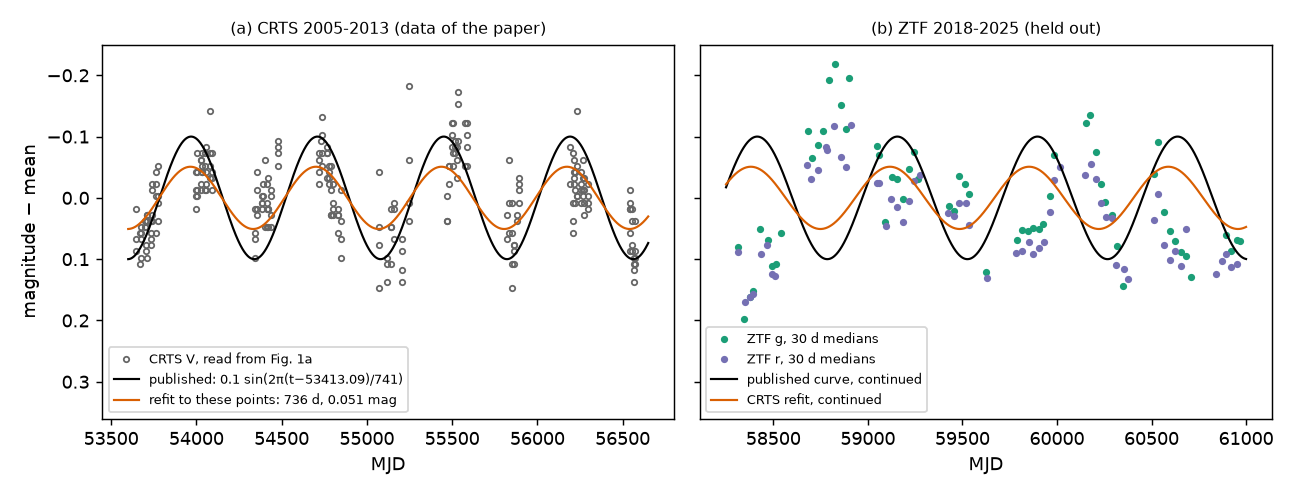
\includegraphics[width=\textwidth]{fig_forecast.png}
\caption{(a) The CRTS V points of Fig.~1a of Zheng et al.\ (one outlier more than 0.3~mag from the median not shown), the published curve (black) and our refit to these points (orange; 736~d, 0.051~mag). (b) ZTF g and r data, 30-day medians after the object offsets are removed, with both curves continued. Brighter is up.}
\label{fig:lc}
\end{figure}

\section{Post hoc tests}
\label{sec:posthoc}

The verification stage of our pipeline asked two questions after the registered result. First, does the published formula describe the paper's own data? Second, does the result exclude a real sinusoid near 741~d, when the uncertainty of the period is taken into account? The formula gives no period error. We wrote the rules of the following tests in a dated addendum to the protocol (Addendum~1). We wrote it after we saw the registered result and the verification stage's first numbers. These tests are therefore post hoc, and their thresholds are not independent of those numbers.

\subsection{CRTS control}

On the 252 CRTS points (unweighted, one offset), the coefficient of the published template is $T_{\rm CRTS} = 0.50$ (0.48 without one point that lies more than 0.3~mag from the median; we remove this point in the fits below). The best sinusoid at 741~d has an amplitude of 0.050~mag and lies 0.010 cycle from the published phase. The best period in 600 to 900~d is 736~d, with an amplitude of 0.051~mag. The residual sum of squares is 0.6196 at the best period, 0.6199 at 741~d and 1.0070 for a constant. So the paper's own points agree with the published period and phase, but they give half of the published amplitude.

This has a consequence for the registered result. The published amplitude of 0.1~mag already disagrees with the CRTS data. The amplitude part of the ZTF failure is therefore not new information. The new information from ZTF is the sign of $T$. If we scale the template to the CRTS amplitude ($T = 0.51$) and keep the period at 741~d, the registered test still gives $\psig = 0.0002$ (1 of 5000). Its power at this amplitude is only 0.25. The rejection still holds because $\Tobs$ is negative.

The CRTS residuals from the refit have an rms of 0.050~mag. The rms of the residuals inside one night is 0.036~mag. We take this as the white noise of CRTS. The remaining red-noise rms is then $\sigma_c = 0.035$~mag.

\subsection{Refit forward test}

A period fitted to four cycles has an error. Over the long gap to ZTF, a small period error becomes a large phase error. This test includes that error. The statistic $C$ is the weighted least-squares coefficient of the ZTF data (with object offsets) on the continued CRTS refit. The refit is the best sinusoid on the CRTS points with free amplitude, phase and offset, at the period with the smallest residual sum of squares on a grid from 600 to 900~d in steps of 2~d. $C = 1$ means that ZTF follows the continued refit. On the real data, $\Cobs = -1.12$.

In each mock, a sinusoid with the published period and phase and amplitude $A$ is present at all times. We add one DRW realization to the CRTS epochs and an independent one to the ZTF epochs, because the gap between them is many times $\tau$. We add white noise: 0.036~mag for CRTS, and each point's error for ZTF. We then refit the mock CRTS light curve and compute $C$ for the mock ZTF data. The grid has eight worlds: $A \in \{0.1, 0.051\}$~mag, CRTS red-noise rms $\sigma_c \in \{0.035, 0.089\}$~mag, and $\tau \in \{210, 500\}$~d. Each world has 2000 mocks. $\ppers$ is the fraction of mocks with $C \le \Cobs$. The rule of the addendum: a persistent sinusoid at the published period and phase is refuted only if $\ppers < 0.01$ in all eight worlds.

\begin{table}[h]
\centering
\caption{Refit forward test (post hoc). 2000 mocks per world. ``sd $\hat P$'' is the scatter of the refitted period. The last column gives the binomial Monte Carlo error of $\ppers$.}
\label{tab:refit}
\begin{tabular}{ccccccc}
\toprule
$A$ (mag) & $\sigma_c$ (mag) & $\tau$ (d) & sd $\hat P$ (d) & $C$ 1\% / 50\% / 99\% & $\ppers$ & error \\
\midrule
0.100 & 0.035 & 210 & 18 & $-1.20$ / $0.89$ / $1.93$ & 0.0135 & 0.0026 \\
0.100 & 0.035 & 500 & 15 & $-0.98$ / $0.93$ / $1.71$ & 0.0055 & 0.0017 \\
0.100 & 0.089 & 210 & 43 & $-1.79$ / $0.25$ / $1.86$ & 0.073 & 0.006 \\
0.100 & 0.089 & 500 & 35 & $-1.53$ / $0.56$ / $1.70$ & 0.054 & 0.005 \\
0.051 & 0.035 & 210 & 35 & $-2.19$ / $0.42$ / $2.50$ & 0.0975 & 0.007 \\
0.051 & 0.035 & 500 & 29 & $-1.77$ / $0.56$ / $2.23$ & 0.081 & 0.006 \\
0.051 & 0.089 & 210 & 72 & $-2.18$ / $-0.02$ / $2.20$ & 0.085 & 0.006 \\
0.051 & 0.089 & 500 & 61 & $-1.75$ / $0.01$ / $1.79$ & 0.064 & 0.005 \\
\midrule
0 (null) & 0.035 & 210 & 106 & $-4.44$ / $-0.03$ / $5.16$ & 0.204 & 0.009 \\
\bottomrule
\end{tabular}
\end{table}

Table~\ref{tab:refit} gives the result. $\ppers$ is between 0.0055 and 0.0975. Only one world is below 0.01. So by the rule of the addendum, a persistent sinusoid is not refuted. The two worlds near 0.01 use the published amplitude of 0.1~mag, which the CRTS points do not support. The four worlds with the CRTS amplitude give 0.064 to 0.098. The values near 0.01 rest on few mocks: 0.0055 is 11 of 2000 mocks and 0.0135 is 27. The verification stage ran the 0.1~mag worlds again with its own code, another seed and 3000 mocks. It obtained 0.0153, 0.0077, 0.080 and 0.057. With both seeds, one of the eight worlds is below 0.01.

The scatter of the refitted period explains the change from the registered test. The phase error at the ZTF epochs is approximately $\Delta t\,\sigma_P/P^2$, where $\Delta t$ is the time from the mean CRTS epoch (MJD 55009.5) to the ZTF epoch. $\Delta t$ is 4.4 to 8.0 cycles of 741~d. With $\sigma_P = 15$~d this gives 0.09 to 0.17 cycle. With $\sigma_P = 72$~d it gives 0.43 to 0.78 cycle. A phase error of this size can turn a correct sinusoid into an anti-phase continuation.

With no sinusoid ($A = 0$), 20\% of mocks give $C \le \Cobs$. So the ZTF data give no evidence for the signal either.

\subsection{Period scan with a CRTS refit}

For each period $P$ from 680 to 810~d in steps of 10~d, we fitted the CRTS points at that fixed $P$ and computed $C$ on ZTF (Table~\ref{tab:scan}). $C$ is negative for 700 to 770~d and positive for 690~d or less and for 780~d or more. A period of 780 to 790~d fits the CRTS points with a residual sum of squares 5\% to 8\% above the minimum and continues to ZTF with $C = 0.7$ to 1.1. We do not claim such a period. The scan only shows that the CRTS data do not fix the period well enough to predict the ZTF phase.

\begin{table}[h]
\centering
\caption{Period scan with a CRTS refit at each period (post hoc).}
\label{tab:scan}
\footnotesize\setlength{\tabcolsep}{3pt}
\begin{tabular}{l*{14}{c}}
\toprule
$P$ (d) & 680 & 690 & 700 & 710 & 720 & 730 & 740 & 750 & 760 & 770 & 780 & 790 & 800 & 810 \\
\midrule
$C$ & 1.05 & 0.66 & $-0.27$ & $-1.30$ & $-1.35$ & $-1.15$ & $-1.15$ & $-1.39$ & $-1.58$ & $-0.45$ & 0.70 & 1.07 & 1.24 & 1.36 \\
RSS & .681 & .665 & .652 & .638 & .627 & .621 & .620 & .623 & .630 & .638 & .650 & .666 & .687 & .713 \\
\bottomrule
\end{tabular}
\end{table}

\subsection{Free-phase amplitude on ZTF}

The ZTF sinusoid at 741~d with free phase has an amplitude of 0.060~mag. Against DRW mocks ($\tau = 210$~d, 2000 mocks), red noise alone gives an amplitude this large in 19\% of mocks. A sinusoid of 0.1~mag at a random phase, plus red noise, gives an amplitude this small in 7.6\% of mocks. A sinusoid of 0.051~mag does so in 48\%. So ZTF cannot exclude a signal of the CRTS size at a shifted phase.

\section{How the result was checked}
\label{sec:prior}

\begin{itemize}
\item \textbf{Order of steps.} The protocol commit precedes the first commit that contains ZTF results. The addendum commit precedes the commit of its numbers. The registered part of the protocol has no changes after its commit; the addendum only adds text.
\item \textbf{Rerun.} \texttt{checks/rerun.py} downloads the ZTF light curves and the arXiv source, recomputes every number in this paper, and compares the numbers with \texttt{data/expected.json}. The verification stage ran it from a clean copy with new downloads, and it printed \texttt{OK}. Both downloads had the stored SHA-256 checksums.
\item \textbf{Independent code.} The verification stage wrote its own code for the registered statistic, the CRTS extraction and the refit worlds. Its CRTS points agree with ours to 0.0005~d and 0.00005~mag. Its refit-world fractions are given above.
\item \textbf{Source quote.} The quoted formula is line 303 of the file \texttt{ms.tex} in the arXiv source of Zheng et al.
\item \textbf{Prior work.} We searched the two public archives of AI-produced results and GitHub issues with the tool \texttt{archive-search} for ``J0159+0105'', ``1512.08730'' and related terms, read the titles of all 38 citing works in Semantic Scholar and all 82 in OpenAlex (2026-11-28), searched the full text of five citing works from 2024 to 2026 that analyse light curves of candidates for the object name, and ran web searches for the object name with ``ZTF'', ``periodic'' and ``741 day''. We found no forward test or reanalysis of J0159 with data after 2013. We did not run a full-text search in the NASA Astrophysics Data System (ADS), so a test outside these indexes is not excluded.
\end{itemize}

\section{Limits}
\label{sec:scope}

\begin{itemize}
\item The CRTS points come from the paper's figure, not from the CRTS archive. Points clipped at the plot edges are missing, so our CRTS data end at MJD 56571, 20~d before those of the paper. The figure has no per-point errors, so the CRTS fits are unweighted.
\item The refit model is least squares with a free period from 600 to 900~d. It is not the GLSdeDRW method of the paper.
\item ZTF g and r are not CRTS V. Quasars usually vary more in bluer bands. The object offsets absorb only constant shifts. Both bands give $T < 0$.
\item The noise model uses one DRW time scale and one rms for both ZTF bands.
\item All tests of Section~\ref{sec:posthoc} are post hoc. Their rules were written after the registered result and the verification stage's first numbers were seen.
\item The IRSA service does not name the ZTF data release in its output. The IRSA web page listed Data Release 24 as the newest on the access date. That the service used this release is not confirmed.
\item We test only the 741-day sinusoid. The 1497-day signal of the autocorrelation analysis, which Zheng et al.\ take as the orbital period, is not tested, because the paper gives no curve for it.
\item We did not run a full-text search in ADS. A forward test of J0159 outside the indexes of Section~\ref{sec:prior} is not excluded.
\end{itemize}

\section{Conclusion}

The literal published formula for the 741-day signal of SDSS J0159+0105 does not continue into 2018--2025. ZTF data run in anti-phase with it ($T = -0.59$, $\psig < 2\times10^{-4}$, registered). Part of this failure is in the original data: the CRTS points of the paper give half of the published amplitude. When the period-fit error of the CRTS data is included, a persistent sinusoid near 741~d is consistent with ZTF in 0.6\% to 9.8\% of simulations (post hoc), so it is not refuted. ZTF does not show the signal either: red noise alone matches the observed result in 20\% of simulations. A sharper test needs a period with a smaller error, for example from a joint fit to CRTS and ZTF with a fixed rule, and later data to test it on.

\section*{Data and code}
ZTF light curves: NASA/IPAC Infrared Science Archive, accessed 2026-11-28. arXiv source of Zheng et al.: \url{https://arxiv.org/src/1512.08730}, accessed 2026-11-28. Code, protocol and expected values: the folder of this result (\texttt{checks/}, \texttt{PROTOCOL.md}, \texttt{data/expected.json}). This work uses data from the Zwicky Transient Facility, obtained through the NASA/IPAC Infrared Science Archive (IRSA).

\begin{thebibliography}{99}
\bibitem{bellm2019} E.~C. Bellm et al., The Zwicky Transient Facility: System Overview, Performance, and First Results, \emph{PASP} \textbf{131}, 018002 (2019), doi:10.1088/1538-3873/aaecbe.
\bibitem{charisi2018} M.~Charisi, Z.~Haiman, D.~Schiminovich, D.~J. D'Orazio, Testing the relativistic Doppler boost hypothesis for supermassive black hole binary candidates, \emph{MNRAS} \textbf{476}, 4617 (2018), doi:10.1093/mnras/sty516, arXiv:1801.06189.
\bibitem{dorazio2023} D.~J. D'Orazio, M.~Charisi, Observational Signatures of Supermassive Black Hole Binaries, arXiv:2310.16896 (2023).
\bibitem{drake2009} A.~J. Drake et al., First Results from the Catalina Real-Time Transient Survey, \emph{ApJ} \textbf{696}, 870 (2009), doi:10.1088/0004-637X/696/1/870.
\bibitem{elbadry2026} K.~El-Badry, D.~W. Hogg, H.-W. Rix, Active Galactic Nuclei Do Not Exhibit Strictly Sinusoidal Brightness Variations, \emph{PASP} \textbf{138}, 024102 (2026), doi:10.1088/1538-3873/ae3f56, arXiv:2509.10601.
\bibitem{graham2015} M.~J. Graham et al., A systematic search for close supermassive black hole binaries in the Catalina Real-time Transient Survey, \emph{MNRAS} \textbf{453}, 1562 (2015), doi:10.1093/mnras/stv1726.
\bibitem{kelly2009} B.~C. Kelly, J.~Bechtold, A.~Siemiginowska, Are the Variations in Quasar Optical Flux Driven by Thermal Fluctuations?, \emph{ApJ} \textbf{698}, 895 (2009), doi:10.1088/0004-637X/698/1/895.
\bibitem{macleod2010} C.~L. MacLeod et al., Modeling the Time Variability of SDSS Stripe 82 Quasars as a Damped Random Walk, \emph{ApJ} \textbf{721}, 1014 (2010), doi:10.1088/0004-637X/721/2/1014.
\bibitem{masci2019} F.~J. Masci et al., The Zwicky Transient Facility: Data Processing, Products, and Archive, \emph{PASP} \textbf{131}, 018003 (2019), doi:10.1088/1538-3873/aae8ac.
\bibitem{vaughan2016} S.~Vaughan et al., False periodicities in quasar time-domain surveys, \emph{MNRAS} \textbf{461}, 3145 (2016), doi:10.1093/mnras/stw1412.
\bibitem{zheng2016} Z.-Y. Zheng, N.~R. Butler, Y.~Shen et al., SDSS J0159+0105: A Radio-Quiet Quasar with a Centi-Parsec Supermassive Black Hole Binary Candidate, \emph{ApJ} \textbf{827}, 56 (2016), doi:10.3847/0004-637X/827/1/56, arXiv:1512.08730.
\end{thebibliography}

\end{document}
